\section{Descrizione Delete}

\paragraph{Descrizione}
Il comando Del, rimuove il primo nodo il cui valore è uguale al parametro passato,
se esiste, altrimenti non altera la lista.

\paragraph{Implementazione}
La funzione scorre tutta la lista finchè non arriva alla fine, oppure finchè non trova
un nodo con il valore da cancellare. Una volta trovato il nodo si distunguono 4 casi:
\begin{itemize}
    \item Il nodo è l'ultimo nodo della lista, in questo caso si imposta il valore 
    del penultimo nodo a -1, in questo modo diventa l'ultimo.
    \item Il nodo non è l'ultimo nodo della lista, in questo caso dobbiamo impostare 
    i puntatori del nodo precedente e del nodo successivo come mostrato in Figura~\ref{fig:delmiddle}.
    \item Il nodo è il primo elemento della lista, in questo caso dobbiamo definire il nodo 
    successivo come primo elemento della lista, aggiornado il puntatore al primo elemento 
    della lista e mettendo il puntatore al nodo precedente del nuovo primo elemento.
    \item Il nodo è l'unico elemento della lista, bisogna ritornare allo stato iniziale 
    del programma mettendo a 0 il puntatore al primo elemento.
\end{itemize}

\begin{figure}[h]
    \centering
    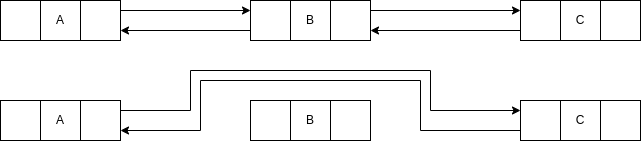
\includegraphics[scale=0.4]{diagrams/del-middle.png}
    \caption{Prima e dopo rimozione di B}
    \label{fig:delmiddle}
\end{figure}

\paragraph{nota} I nodi non vengono effettivamente cancellati dalla memoria, 
semplicemente non vengono più indicizzati dalla lista. Un miglioramento potrebbe 
essere fatto azzerando la memoria dei nodi cancellati in modo da poter riusare lo 
spazio in memoria.